\section{Run 3}
For this last approach we decided to implement \textbf{transfer learning}: this means that in order to extract significant features from our images we used layers of a pre-trained neural network. So, to complete our classification architecture, we re-trained just the last layers used for classification on our training set, without doing backpropagation on the previous layers. Surely one advantage of this solution is that allowed us to save a considerable amount of computational time for the training of all the layers of the network.

For this particular problem we decided to use the convolutional neural network (CNN) \code{alexnet}, winner of the 2012 ImageNet Large Scale Visual Recognition Challenge (ILSVRC2012). At the time, it takes an entire week to train the complete network with the competition dataset (1.2M of images).

The main difference with respect to standard NN is that in CNNs neurons are arranged in three spatial dimensions, and so they take 3D inputs and return 3D outputs. This is the main peculiarity that allows CNN performing so good and being so fast: we can clearly see the advantage if we have manipulate RGB images, which have 3 different layers (\textit{Red, Green} and \textit{Blue}), instead of grayscale ones. 

Delving more into some details of \code{alexnet}, we can subdivide its layers in the following types:
\begin{itemize}
	\item INPUT: it accepts 227x227x3 images, so we wrote \code{preprocessingFcn} to resize the images when importing them from the datastore.
	\item CONVOLUTIONAL: it consists of a set of 3D convolutional filters used to actually extract features from the image; each different convolutional layer in the network extracts a set of different features, depending on the characteristics of the filter.
	\item ReLU: it applies the $max(0,x)$ \textbf{activation function} to the output of the convolutional layer; these types of layer in particular are involved in backpropagation, when the network is initially trained.
	\item POOL: it performs downsampling (useful when the work has to be split between two different workers, as during the training of \code{alexnet})
	\item FC (fully connected): refined features comes out from this layer.
\end{itemize}

In our case, we chopped off the network on the $20^{th}$ layer; so, we use features extracted from layer \code{fc7}. All the code of this part can be found in \code{featuresExtractionNetwork}. 

After that, we used the features from the training set to train our classifier. Specifically we used an error-correcting output codes (ECOC) classifier, particularly good when it comes to multiclass learning: it proceeds by reducing the problem to multiple binary classifiers (thanks to coding strategies) such as Support Vector Machines (which we used in our configuration). 

We tested different coding designs (which determine the policy used to reduce the structure to binary learners) on the validation set, obtaining the accuracy values listed in Table 1. Of course the more complex is one strategies, more time it takes to train the classifier. 

\begin{table}[h]
	\centering
	\begin{tabular}{|c|c|c|}
		\hline
		\textbf{Coding Strategy}  & \textbf{Accuracy} \\ \hline
		One VS All & 0.8427           \\ \hline
		One VS One & 0.8400 \\ \hline
		Ordinal & 0.6960 \\ \hline
		Sparse Random & 0.8283 \\ \hline
	\end{tabular}
	\caption{Accuracy with different coding strategies}
	\label{tab:MSE}
\end{table}

We found our best results using \code{onevsall} and we decided to implement it also with our final predictions; looking to the confusion matrix in Figure \ref{fig:heat} we can notice more in detail errors made from the classifier. For example, \textit{Coast} has been misclassified twice with \textit{OpenCountry} while \textit{Bedroom} has been mostly misclassified with \textit{LivingRoom}. This suggests us that our architectureis vulnerable when dealing with images that could have really similar features.  

\begin{figure}[!htbp] 
	\centering
	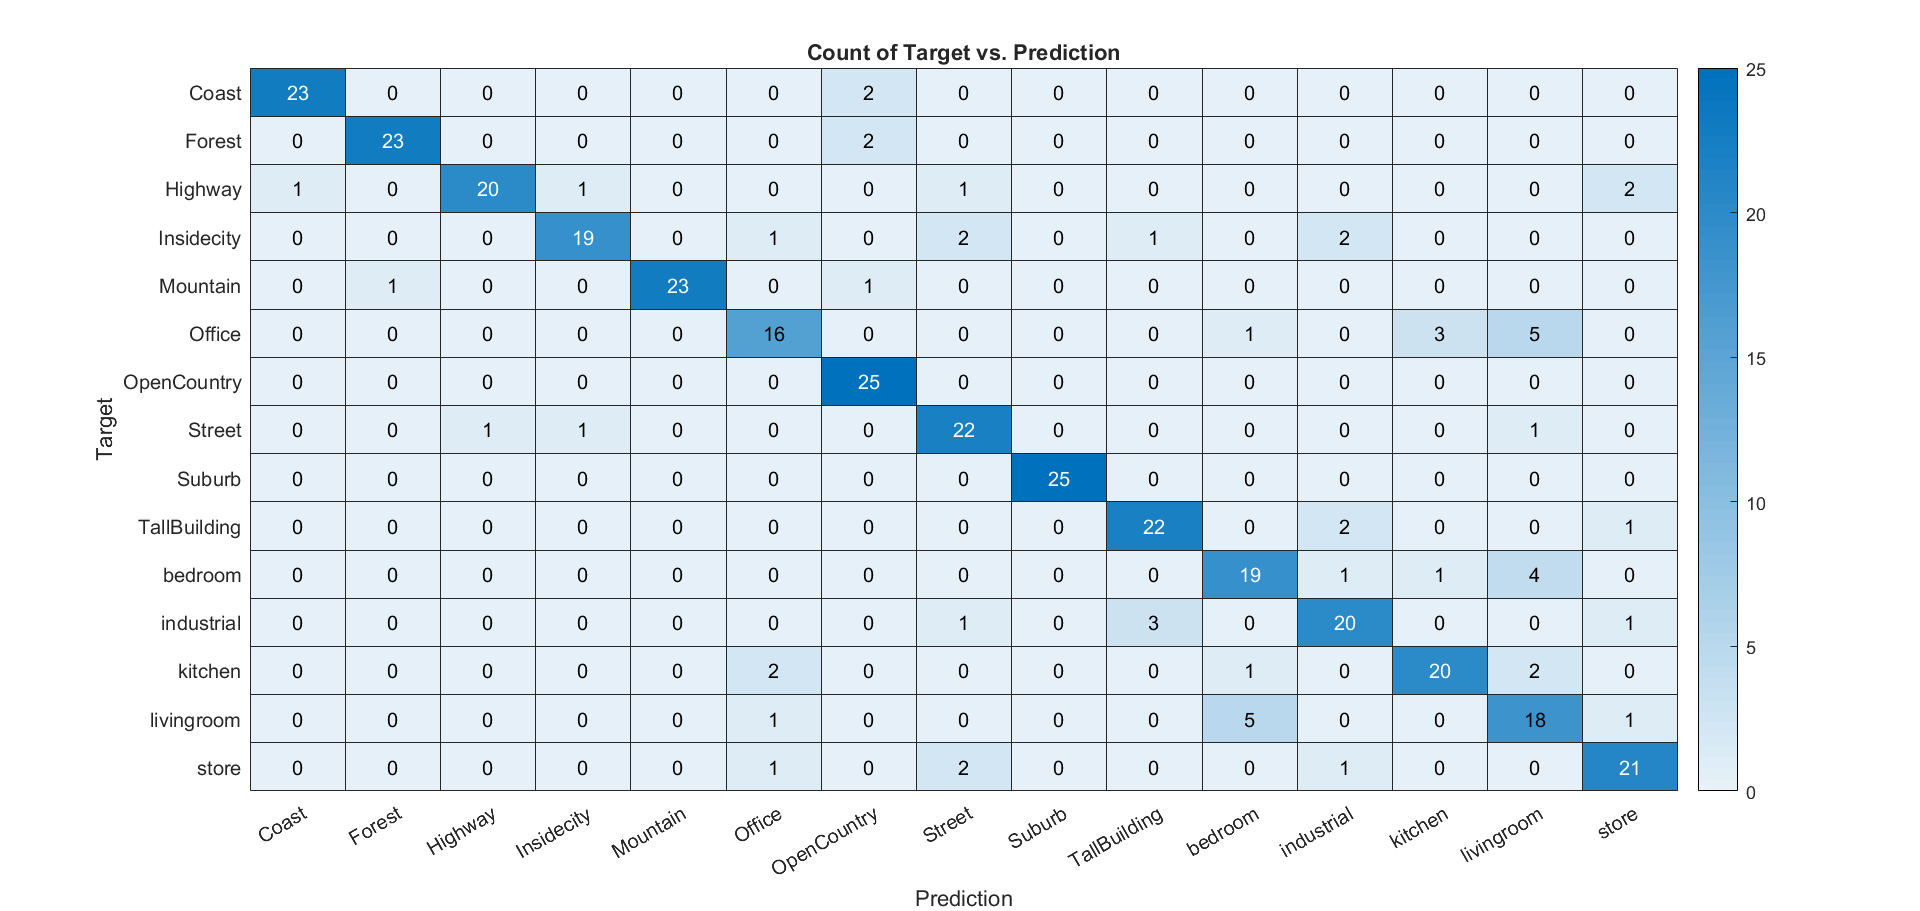
\includegraphics[width=1\linewidth]{img/heatmap}
	\caption{Confusion matrix obtained with one-vs-all coding design}
	\label{fig:heat}
\end{figure}